\documentclass[12pt]{article}
\usepackage{graphicx}
\usepackage[bulgarian]{babel}
\usepackage[utf8]{inputenc}

\textwidth 170mm
\textheight 210mm
\oddsidemargin 5mm
\evensidemargin 5mm

\begin{document}

\begin{center}
\textbf{\Large Софтуер "НЦРРЗ Комети"}\\[10pt]
 (версия 0.3/25.09.2005)\\[10pt]
 \textbf{Кирил Киров, Николай Киров}\\
 \verb|k.n.kirov@gmail.com, nkirov@math.bas.bg|
\end{center}

 Системата е предназначена за обработка на изображения, получени по технология на НЦРРЗ и
 пресмятане на числови характеристики за всяка комета от
 изображението.

 Входният файл е сиво (gray-scale) точково (bitmap) изображение с размери $X$ на $Y$,
 т.е. за точка от изображението $(x,y)$ (с цели координати),
 $0\leq x < X, 0\leq y < Y$, за стойността на пиксела $p_{xy}$ в тази точка
 имаме $0\le p_{xy} < 256$.

1. Генерира се хистограма $\{h_i\}_{i=0}^{255}$ с разпределението на
стойностите на точките на цялото изображение.
$$
 h_i = | \{(x,y):  p_{xy} = i \} |,\ \ \mbox{т.е. $h_i$ е броят на точките със стойност} \ i.
$$
Определя се средна стойност на фона $a$:
$$
 h_m = \max_{i \in [0,255]} \{h_i\}, \ \ a =  m + k,
$$
където $k$ е константа (в тази версия $k = 10$). За точки от комета
се считат всички точки със стойност по-голяма от средната стойност
на фона $a$.

2. Отделят се кометите, като най-напред се намира центърът на
главата на кометата -- точка $(x_0, y_0)$ с най-голяма стойност
(локален
максимум). След това по хоризон\-тал (наляво-надясно) --
до намиране на точка от фона (със стойност по-малка от $a$) --
се определя дължината на кометата.
После по цялата дължина се търси по вертикал
(нагоре-надолу) точка от фона, за да се определи ширината на кометата.
Така за всяка комета се
определя правоъгълник, съдържащ кометата. След това се премахват
всички комети с пресичащи се право\-ъгъл\-ници. Така всяка комета се
определя от 6 числа: $x_{\min}$, $x_{\max}$, $y_{\min}$,
$y_{\max}$ и координатите на центъра на главата $x_0$ и $y_0$.

3. Да означим с $P$ множеството от всички точки,
 принадлежащи на правоъгълника на кометата, т.е.
$$
 P = \{ (x,y): x_{\min} \leq x \le x_{\max} \ \mbox{и}\
 y_{\min} \leq y \le y_{\max} \}.
$$
Точките на кометета формират множеството
$$
  C = \{ (x,y): (x,y) \in P \ \ \mbox{и}\ \ p_{xy} > a \},
$$
 т.е. точки със стойност по-голяма от средната стойност
 на фона в правоъгълника на кометата.

Кометата се състои от глава (head) и опашка (tail).

Да означим с $P_h$ множеството от всички точки,
принадлежащи на правоъгълника, определен от
началото на кометата и центъра на главата, т.е.
$$
 P_h = \{ (x,y): x_{\min} \leq x \le x_0 \ \mbox{и}\
 y_{\min} \leq y \le y_{\max} \}.
$$
Радиусът на главата е $r_h = x_0 - x_{\min}$. Точките на кометата в
дефинирания правоъгълник $P_h$ са половината от точките на главата
на кометата:
$$
  C_h = \{ (x,y): (x,y) \in P_h \ \ \mbox{и}\ \ p_{xy} > a \}.
$$
Смятаме, че другата половина на главата на кометата е огледален образ на
първата половина.

Да означим с $P_{ht}$ множеството от всички точки,
принадлежащи на правоъгълника, определен от
центъра на главата и края на главата, т.е.
$$
 P_{ht} = \{ (x,y): x_0 \leq x \le x_0 + r_h  \ \ \mbox{и}\
 y_{\min} \leq y \le y_{\max} \}.
$$
Този правоъгълник съдържа точки и от главата и от опашката на кометата:
$$
  C_{ht} = \{ (x,y): (x,y) \in P_{ht} \ \ \mbox{и}\ \ p_{xy} > a \}.
$$

Да означим с $P_t$ множеството от всички точки,
 принадлежащи на правоъгълника на кометата и непринадлежащи на
другите два правоъгълника:
$$
 P_t = P \backslash \left(P_h \cup P_{ht}\right).
$$
Точките на кометата в правоъгълника $P_t$ са точки от опашката на кометата
$$
  C_t = \{ (x,y): (x,y) \in P_t \ \ \mbox{и}\ \ p_{xy} > a \}.
$$

4. Определят се характеристиките на всяка комета, следвайки
 дефинициите на \cite{1}.

\textbf{За кометата:}
\begin{itemize}
\item
 Дължина (Comet Length):
$$
 x_c = x_{\max} - x_{\min};
$$
\item
 Височина (Comet Height):
$$
 y_c = y_{\max} - y_{\min};
$$
\item
 Площ (Comet Area):
$$
 a_c = | C |,\ \ \textrm{брой на точките на множеството} \ \ C;
$$
\item
 Обща интензивност (Total Comet Intensity):
$$
 i_c = \displaystyle\sum_{(x, y)\in C}p_{xy};
$$
\item
 Средна интензивност (Mean Comet Intensity):
$$
m_c = \displaystyle\frac{i_c}{a_c}.
$$
\end{itemize}

\textbf{За главата на кометата:}
\begin{itemize}
\item
 Диаметър (Head Diameter):
$$
 d_h = 2r_h;
$$
\item
 Площ (Head Area):
$$
 a_h = 2 | C_h |;
$$
\item
 Обща интензивност (Total Head Intensity):
$$
 i_h = 2\sum_{(x, y)\in C_h} p_{xy};
$$
\item
 Средна интензивност (Mean Head Intensity):
$$
 m_h = \frac{i_h}{a_h};
$$
\item
 Процент на ДНК (\% DNA in Head):
$$
 D_h = 100 \frac{i_h}{i_c}.
$$
\end{itemize}

\textbf{За опашката на кометата:}
\begin{itemize}
\item
 Дължина (Tail Length):
$$
 x_t = x_c - d_h;
$$
\item
 Площ (Tail Area):
$$
 a_t = | C_t |;
$$
\item
 Обща интензивност (Total Tail Intensity):
$$
 i_t = \left(\sum_{(x, y)\in C_{th} \cup C_t} p_{xy}\right) - \frac{i_h}2
 = \sum_{(x, y)\in C}\ \textrm{sign}(x - x_0) p_{xy};
$$
\item
 Средна интензивност (Mean Tail Intensity):
$$
 m_t = \displaystyle\frac{i_t}{a_t};
$$
\item
 Процент на ДНК (\% DNA in Tail):
$$
 D_t = 100 \frac{i_t}{i_c};
$$
\item
 Момент (Tail Moment):
$$
 M_t = \frac{D_t x_t}{100} =  \frac{i_t x_t}{i_c};
$$
\item
 Момент на размазване (Olive Moment):
$$
 M_o = \frac1{i_c}\sum_{x = x_{\min}}^{x_{\max}} (x - x_0)
  \sum_{y = y_{\min}}^{y_{\max}} p_{xy} =
\frac1{i_c} \sum_{(x,y)\in C} p_{xy}.
$$
\end{itemize}

Програмата създава текстов файл, съдържащ числовите характеристики
на всички намерени комети в изображението - входен файл.


\begin{thebibliography}{qq}
\bibitem{1}
 CometScore$^{\mbox{\small TM}}$, TriTek Corp.
 \verb|http://autocomet.com/home.php|
\bibitem{2}
 COMET ASSAY FORUM,
 \verb|http://www.comet.itrcindia.org/introduction.htm|
\end{thebibliography}

%\bigskip
\newpage
{\bf\large Приложение 1. Използване на програмата \verb|com03|.}

\medskip
Данните за програмата и резултатите от работата и се съхраняват в
папка \verb|img|. Вход\-ни\-ят файл е сиво (gray-scale) изображение
във \verb|pgm| графичен формат. Програмата се стартира с:
\begin{verbatim}
...>com03 <file>
\end{verbatim}

Например:
\begin{verbatim}
C:\comets>com03 gy1a
\end{verbatim}
чете файл \verb|img\gy1a.pgm|.

 Програмата произвежда следните файлове:

\begin{itemize}
\item
 Текстов файл с числата от хистограмата
 за разпределение на стойностите на точките на изображението
 (\verb|gy1a.txt|);
\item
 Графичен файл с хистограмата за разпределение на стойностите
 на точките на изображението
 (\verb|gy1a_h.pgm|, даден на Фиг.\,\ref{Fig1});
\item
 Входният графичен файл с обозначени правоъгълниците на намерените
 комети, с пресичания на правоъгълници
 (\verb|gy1a_1.pgm|);
\item
 Входният графичен файл с обозначени правоъгълниците на намерените
 комети, без пресичания на правоъгълници
 (\verb|gy1a_2.pgm|, даден на Фиг.\,\ref{Fig1});
 \begin{figure}[b]
  % Requires \usepackage{graphicx}
 \center {\fbox{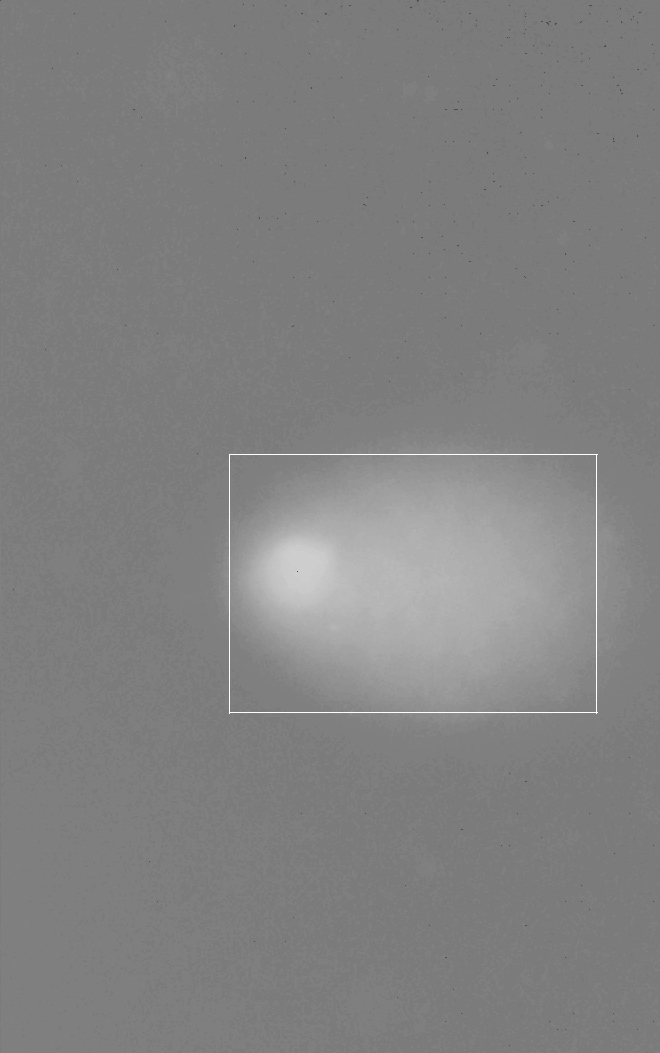
\includegraphics[width=8cm]{gy1a_2.jpg}}\hfill
          \fbox{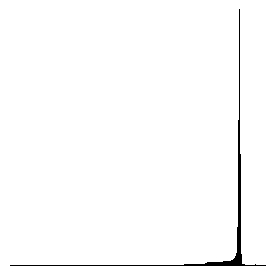
\includegraphics[width=8cm]{gy1a_h.jpg}}}
  \caption{}
  \label{Fig1}
\end{figure}
\item
 Текстов файл с броят на точките на комета, лежащи на вертикалните
 отсечки с краища $y_{\min}$ и $y_{\max}$ за всяко $x \in [x_{\min},
 x_{\max}]$. Файлът съдържа данни за всички намерени комети, като преди
 числата за кометата е даден поредният и номер\linebreak
 (\verb|gy1a_b.txt|);
\item
 Графичен файл с хистограма на броят на точките на комета, лежащи на вертикалните
 отсечки с краища $y_{\min}$ и $y_{\max}$ за всяко $x \in [x_{\min},
 x_{\max}]$. Дадени са отделни графики за главата и опашката на
 кометата (\verb|gy1a_b.pgm|, даден на Фиг.\,\ref{Fig3});
 \begin{figure}[b]
  % Requires \usepackage{graphicx}
 \center {\fbox{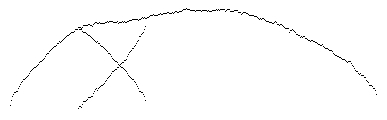
\includegraphics[width=10cm]{gy1a_b.jpg}}}
     \caption{}
  \label{Fig3}
\end{figure}
\item
 Текстов файл с параметрите на намерените комети. Първият ред
 на файла се състои от името на файла, следват по 18 реда за всяка
 комета. Най-напред е поредният номер на кометата във файла, числата
 $x_{\min}$-$x_{\max}$ : $y_{\min}$-$y_{\max}$ и след това
 параметрите на кометата, както са описани по-горе
 (\verb|gy1a_c.txt|, даден на Фиг.\,\ref{Fig2});
 \begin{figure}[t]
 \center {
\begin{verbatim}
 gy1a
 No. 0 229-597 : 454-713
 Comet Length          368
 Comet Height          259
 Comet Area            70906
 Total Comet Intensity 3493225
 Mean Comet Intensity  49.2656
 Head Diameter         136
 Head Area             16098
 Total Head Intensity  830412
 Mean Head Intensity   51.5848
 %DNA in Head          23.7721
 Tail Length           232
 Tail Area             49107
 Total Tail Intensity  2662813
 Mean Tail Intensity   54.2247
 %DNA in Tail          76.2279
 Tail Moment           176.849
 Olive Moment          115.204
\end{verbatim}
}
 \caption{}
 \label{Fig2}
\end{figure}
\end{itemize}

\end{document}
